\documentclass{article}

%% Denote paragraphs with vertical space rather than indenting (not critical)
\usepackage{parskip}

%% Support for URL in introductory text (not needed for main example)
\usepackage{url}

%% *** Enable TikZ ***
\usepackage{tikz}


\begin{document}

%% Introductory Text
Example 3.9 from the book\\
\emph{Unlocking LaTeX Graphics: A Concise Guide to Ti$k$Z/PGF and PGFPLOTS}.\\
For more information, visit \url{https://latex-graphics.com}.
\par\bigskip

%% *** START OF EXAMPLE CODE ***
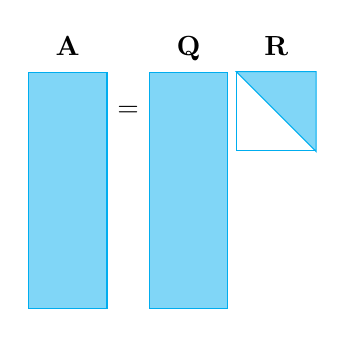
\begin{tikzpicture}[c/.style={cyan,draw,fill=.!50},
    matrix/.style={c,anchor=north west,
      minimum width=1cm, minimum height=3cm},
    matname/.style={anchor=base,yshift=2mm},]
  \node[matrix] (A) {};
  \path (A.north east) node[anchor=west, yshift=-5mm] (eq) {=};
  \path (A.north -| eq.east) node[matrix] (Q) {};
  \path (Q.north east) node[matrix, minimum height=1cm, fill=none, xshift=1mm] (R) {};
  \filldraw[c] (R.north west) -- (R.north east) --(R.south east) -- cycle;
  \node[matname] at (A.north) {$\mathbf{A}$};
  \node[matname] at (Q.north) {$\mathbf{Q}$};
  \node[matname] at (R.north) {$\mathbf{R}$};
\end{tikzpicture}
%% *** END OF EXAMPLE CODE ***

\end{document}
